\documentclass[class=article,crop=false]{standalone}

\usepackage{../setting/preamble_}

\begin{document}
\twocolumn

\section{Methodology}
\subsection{Preliminary Analysis}
At an earlier stage of the project, we plan to build an octave piano with twelve notes including minor keys. At that stage, we analyzed the frequency spectrum of each note and found out it is possible to produce a majority feeling of sound with only four harmonics to a given note. 
\par 
After synthesizing all the keynotes from its harmonics using Matlab, we moved to circuit development. At this stage, we decided to stimulate only one note from the piano because the generation of notes is modularizable. For this purpose, we have chosen the C-wave which is in the middle of the spectrum.
\begin{figure}
    \begin{subfigure}{.45\columnwidth}
        \centering
            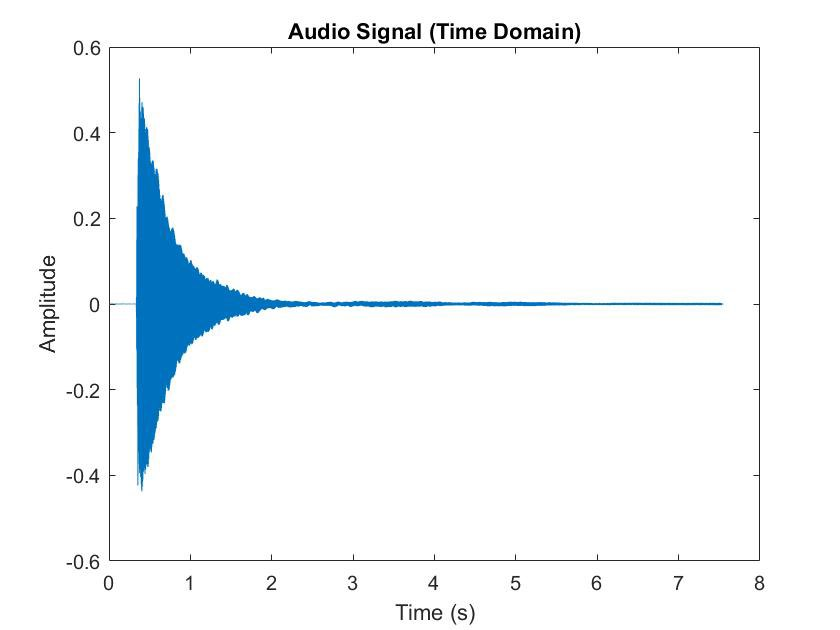
\includegraphics[width=.9\columnwidth]{c_wave}
    \end{subfigure}
    \begin{subfigure}{.45\columnwidth}
        \centering
            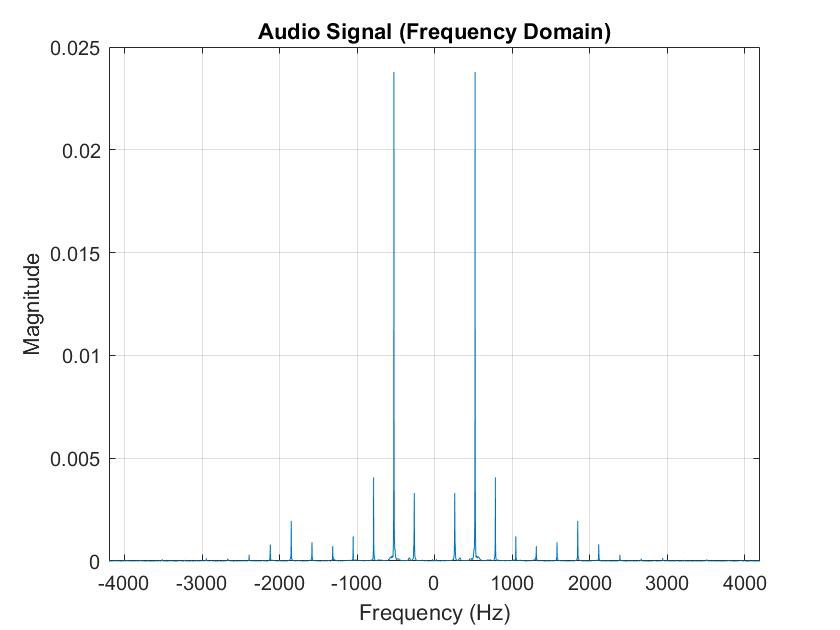
\includegraphics[width=.9\columnwidth]{spectrum_c}
    \end{subfigure}

\end{figure}
\subsection{Circuit Design}

\begin{figure}
    \begin{center}
        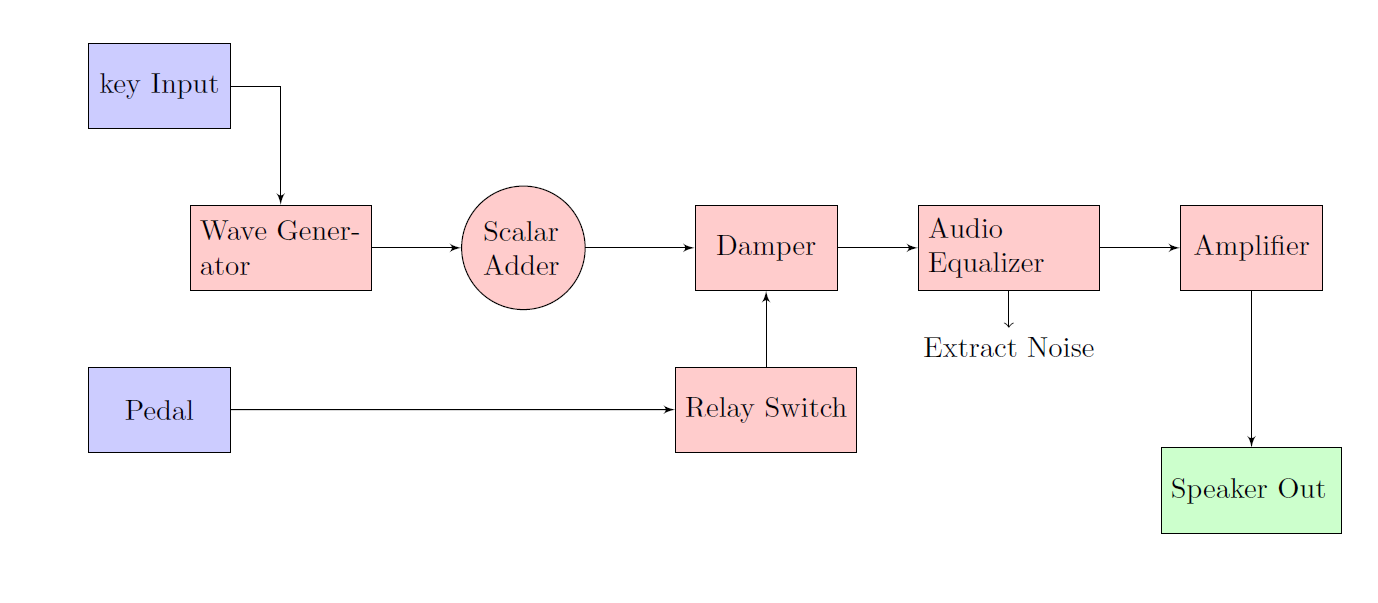
\includegraphics[width=\columnwidth]{flow}
        \caption*{Block Diagram of the Circuit}
    \end{center}
\end{figure}
\subsubsection{Wave Generator}
\subsubsection{Damper}
\subsubsection{Scalar Adder}
\subsubsection{Amplifier}
\end{document}